% tikzpicture starts at line 3180 of input.tex
\documentclass{standalone}

\usepackage{amsthm, amsmath}

% Prevent the eventual "Too many alphabets" error
\newcommand\hmmax{0}
\newcommand\bmmax{0}

\RequirePackage{notomath}
\RequirePackage{inter}
\RequirePackage[scaled=0.85]{DejaVuSansMono}
\def\bfseries@rm{sb}

\DeclareMathVersion{sansmath}
\SetSymbolFont{operators}{sansmath}{OT1}{NotoSans-TLF}{m}{n}
\SetSymbolFont{letters}{sansmath}{OML}{notosansmi}{m}{it}
\SetMathAlphabet\mathbf{sansmath}{OT1}{NotoSans-TLF}{b}{n}
\SetMathAlphabet\mathsf{sansmath}{OT1}{NotoSans-TLF}{m}{n}
\SetMathAlphabet\mathit{sansmath}{OT1}{NotoSans-TLF}{m}{it}

\DeclareMathVersion{sansmathbold}
\SetSymbolFont{operators}{sansmathbold}{OT1}{NotoSans-TLF}{b}{n}
\SetSymbolFont{letters}{sansmathbold}{OML}{notosansmi}{b}{it}
\SetSymbolFont{symbols}{sansmathbold}{LMS}{ntxsy}{b}{n}
\SetMathAlphabet\mathbf{sansmathbold}{OT1}{NotoSans-TLF}{b}{n}
\SetMathAlphabet\mathsf{sansmathbold}{OT1}{NotoSans-TLF}{b}{n}
\SetMathAlphabet\mathit{sansmathbold}{OT1}{NotoSans-TLF}{b}{it}


% Upright Greek letters uppercase
\DeclareMathSymbol{\Gamma}{\mathord}{operators}{0}
\DeclareMathSymbol{\Delta}{\mathord}{operators}{1}
\DeclareMathSymbol{\Theta}{\mathord}{operators}{2}
\DeclareMathSymbol{\Lambda}{\mathord}{operators}{3}
\DeclareMathSymbol{\Xi}{\mathord}{operators}{4}
\DeclareMathSymbol{\Pi}{\mathord}{operators}{5}
\DeclareMathSymbol{\Sigma}{\mathord}{operators}{6}
\DeclareMathSymbol{\Upsilon}{\mathord}{operators}{7}
\DeclareMathSymbol{\Phi}{\mathord}{operators}{8}
\DeclareMathSymbol{\Psi}{\mathord}{operators}{9}
\DeclareMathSymbol{\Omega}{\mathord}{operators}{10}

% Italic Greek letters lowercase
\DeclareMathSymbol{\alpha}{\mathord}{letters}{11}
\DeclareMathSymbol{\beta}{\mathord}{letters}{12}
\DeclareMathSymbol{\gamma}{\mathord}{letters}{13}
\DeclareMathSymbol{\delta}{\mathord}{letters}{14}
\DeclareMathSymbol{\epsilon}{\mathord}{letters}{15}
\DeclareMathSymbol{\zeta}{\mathord}{letters}{16}
\DeclareMathSymbol{\eta}{\mathord}{letters}{17}
\DeclareMathSymbol{\theta}{\mathord}{letters}{18}
\DeclareMathSymbol{\iota}{\mathord}{letters}{19}
\DeclareMathSymbol{\kappa}{\mathord}{letters}{20}
\DeclareMathSymbol{\lambda}{\mathord}{letters}{21}
\DeclareMathSymbol{\mu}{\mathord}{letters}{22}
\DeclareMathSymbol{\nu}{\mathord}{letters}{23}
\DeclareMathSymbol{\xi}{\mathord}{letters}{24}
\DeclareMathSymbol{\pi}{\mathord}{letters}{25}
\DeclareMathSymbol{\rho}{\mathord}{letters}{26}
\DeclareMathSymbol{\sigma}{\mathord}{letters}{27}
\DeclareMathSymbol{\tau}{\mathord}{letters}{28}
\DeclareMathSymbol{\upsilon}{\mathord}{letters}{29}
\DeclareMathSymbol{\phi}{\mathord}{letters}{30}
\DeclareMathSymbol{\chi}{\mathord}{letters}{31}
\DeclareMathSymbol{\psi}{\mathord}{letters}{32}
\DeclareMathSymbol{\omega}{\mathord}{letters}{33}
\DeclareMathSymbol{\varepsilon}{\mathord}{letters}{34}
\DeclareMathSymbol{\vartheta}{\mathord}{letters}{35}
\DeclareMathSymbol{\varpi}{\mathord}{letters}{36}
\DeclareMathSymbol{\varrho}{\mathord}{letters}{37}
\DeclareMathSymbol{\varsigma}{\mathord}{letters}{38}
\DeclareMathSymbol{\varphi}{\mathord}{letters}{39}

% Change font tracking
\RequirePackage[letterspace=150]{microtype}

% Page breaking
\widowpenalty=10000
\clubpenalty=10000

%%%% Author's definition can start here

\usepackage{tikz}
\usepackage{tkz-graph}
\usepackage{mathdots}
\usepackage{dsfont}
\usetikzlibrary{shapes}

\DeclareMathOperator{\spn}{span}
\DeclareMathOperator{\tr}{tr}
\DeclareMathOperator{\rr}{\mathbb{R}}
\DeclareMathOperator{\cc}{\mathbb{C}}
\DeclareMathOperator{\arity}{arity}
\DeclareMathOperator{\vk}{\mathbf{K}}
\DeclareMathOperator{\vl}{\mathbf{L}}
\DeclareMathOperator{\vg}{\mathbf{G}}
\DeclareMathOperator{\vx}{\mathbf{x}}
\DeclareMathOperator{\vy}{\mathbf{y}}
\DeclareMathOperator{\vz}{\mathbf{z}}
\DeclareMathOperator{\va}{\mathbf{a}}
\DeclareMathOperator{\vb}{\mathbf{b}}
\DeclareMathOperator{\vq}{\mathbf{Q}}
\DeclareMathOperator{\vr}{\mathbf{R}}
\DeclareMathOperator{\vrr}{\mathbf{r}}
\DeclareMathOperator{\vc}{\mathbf{C}}
\DeclareMathOperator{\vcc}{\mathbf{c}}
\DeclareMathOperator{\vj}{\mathbf{J}}
\DeclareMathOperator{\vjj}{\mathbf{j}}
\DeclareMathOperator{\ic}{\mathcal{I}}
\DeclareMathOperator{\fc}{\mathcal{F}}
\DeclareMathOperator{\gc}{\mathcal{G}}
\DeclareMathOperator{\gk}{\mathfrak{G}_{\mathcal{F}}}
\DeclareMathOperator{\qk}{\mathfrak{Q}_{\mathcal{F}}}
\DeclareMathOperator{\stab}{Stab}
\newcommand{\tcwd}[1]{\left\langle #1 \right\rangle_{+, \circ, \otimes ,\top}}
\newcommand{\tcwdn}[1]{\left\langle #1 \right\rangle_{\circ, \otimes ,\top}}
\DeclareMathOperator{\holant}{Holant}
\DeclareMathOperator{\plholant}{Pl-Holant}
\DeclareMathOperator{\csp}{\#CSP}
\DeclareMathOperator{\qut}{Qut}
\DeclareMathOperator{\aut}{Aut}
\DeclareMathOperator{\eq}{\mathcal{EQ}}
\DeclareMathOperator{\geneq}{\mathcal{GEQ}}

\renewcommand*{\VertexSmallMinSize}{6pt}
% draw edges with diamonds in tikz
\newcommand{\DEdge}[2]{
    \draw[thick] (#1) -- (#2) node[draw, fill=white, kite, kite vertex angles = 120, minimum size = 4pt, inner sep = 1pt, pos=0.3, sloped] {};
}


\begin{document}
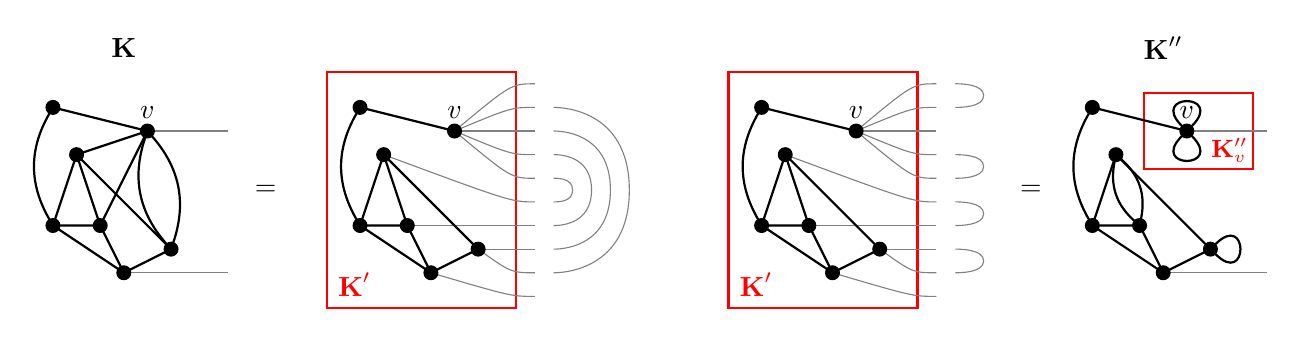
\begin{tikzpicture}[scale=0.6]
    \GraphInit[vstyle=Classic]
    \SetUpEdge[style=-]
    \SetVertexMath
    \tikzset{VertexStyle/.style = {shape=circle, fill=black, minimum size=5pt, inner sep=1pt, draw}}

    % length of dangling edges
    \def\wlen{1.2}
    \def\wgap{0.4}
    \def\yy{0.5}

    % vertex coordinates
    \def\ax{0}
    \def\ay{8*\yy}
    \def\bx{0.5}
    \def\by{6*\yy}
    \def\cx{2}
    \def\cy{7*\yy}
    \def\dx{0}
    \def\dy{3*\yy}
    \def\ex{1}
    \def\ey{3*\yy}
    \def\fx{2.5}
    \def\fy{2*\yy}
    \def\gx{1.5}
    \def\gy{1*\yy}

    % gadget x shifts
    \def\x{0}
    \def\xx{6.5}
    \def\xxx{15}
    \def\xxxx{22}

    \node at (\x+1.5,10.5*\yy) {$\vk$};
    \node at (\xxxx+1.5,10.5*\yy) {$\vk''$};
    \node at (\xx-2,4.5*\yy) {$=$};
    \node at (\xxx-1.8,4.5*\yy) {$\rightsquigarrow$};
    \node at (\xxxx-1.3,4.5*\yy) {$=$};

    \begin{scope}[xshift=\xx cm]
        \node at (-0.12,0.5*\yy) {$\textcolor{red}{\vk'}$};
        \draw[color=red,thick] (-0.7,-0.5*\yy) rectangle (\fx+\wlen-\wgap,9.5*\yy);
    \end{scope}

    \begin{scope}[xshift=\xxx cm]
        \node at (-0.12,0.5*\yy) {$\textcolor{red}{\vk'}$};
        \draw[color=red,thick] (-0.7,-0.5*\yy) rectangle (\fx+\wlen-\wgap,9.5*\yy);
    \end{scope}

    \begin{scope}[xshift=\xxxx cm]
        \node[font=\small] at (\cx+0.9,\cy-0.4) {$\textcolor{red}{\vk''_v}$};
        \draw[color=red,thick] (\cx-0.9,\cy-0.8) rectangle (\cx+1.4,\cy+0.8);
    \end{scope}

    % original K
    \draw[thin, color=gray] (\cx,\cy) -- (\fx+\wlen,\cy);
    \draw[thin, color=gray] (\gx,\gy) -- (\fx+\wlen,\gy);

    % broken K and broken K'' dangling edges
    \foreach \ii/\xsh in {1/\xx,2/\xxx} {
    \begin{scope}[xshift=\xsh cm]
        \draw[thin, color=gray] (\fx+\wlen,9*\yy) .. controls +(-0.5,0) .. (\cx,\cy);
        \draw[thin, color=gray] (\fx+\wlen,8*\yy) .. controls +(-0.5,0) .. (\cx,\cy);
        \draw[thin, color=gray] (\fx+\wlen,7*\yy) .. controls +(-0.5,0) .. (\cx,\cy);
        \draw[thin, color=gray] (\fx+\wlen,6*\yy) .. controls +(-0.5,0) .. (\cx,\cy);
        \draw[thin, color=gray] (\fx+\wlen,5*\yy) .. controls +(-0.5,0) .. (\cx,\cy);
        \draw[thin, color=gray] (\fx+\wlen,4*\yy) .. controls +(-0.5,0) .. (\bx,\by);
        \draw[thin, color=gray] (\fx+\wlen,3*\yy) .. controls +(-0.5,0) .. (\ex,\ey);
        \draw[thin, color=gray] (\fx+\wlen,2*\yy) .. controls +(-0.5,0) .. (\fx,\fy);
        \draw[thin, color=gray] (\fx+\wlen,1*\yy) .. controls +(-0.5,0) .. (\fx,\fy);
        \draw[thin, color=gray] (\fx+\wlen,0*\yy) .. controls +(-0.5,0) .. (\gx,\gy);
    \end{scope}
    }

    % connecting wires for broken K
    \begin{scope}[xshift=\xx cm]
    \foreach \high/\low/\m in {8/1/1.6,7/2/1.2,6/3/0.8,5/4/0.4} {
        \draw[thin, color=gray] (\fx+\wlen+\wgap,\low*\yy) .. controls
        +(0.1,0) and (\fx+\wlen+\wgap+\m,\low*\yy) ..
        (\fx+\wlen+\wgap+\m,{(\high+\low)/2*\yy}) .. controls
        (\fx+\wlen+\wgap+\m,\high*\yy) and +(0.1,0) ..
        (\fx+\wlen+\wgap,\high*\yy);
    }
    \end{scope}

    % connecting wires for broken K''
    \begin{scope}[xshift=\xxx cm]
    \foreach \high/\low/\m in {9/8/0.6,6/5/0.6,4/3/0.6,2/1/0.6} {
        \draw[thin, color=gray] (\fx+\wlen+\wgap,\low*\yy) .. controls
        +(0.1,0) and (\fx+\wlen+\wgap+\m,\low*\yy) ..
        (\fx+\wlen+\wgap+\m,{(\high+\low)/2*\yy}) .. controls
        (\fx+\wlen+\wgap+\m,\high*\yy) and +(0.1,0) ..
        (\fx+\wlen+\wgap,\high*\yy);
    }
    \end{scope}

    % K'' dangling edges
    \begin{scope}[xshift=\xxxx cm]
        \draw[thin, color=gray] (\cx,\cy) -- (\fx+\wlen,\cy);
        \draw[thin, color=gray] (\gx,\gy) -- (\fx+\wlen,\gy);
    \end{scope}


    \foreach \ii/\xsh in {0/\x,1/\xx,2/\xxx,3/\xxxx} {
        \begin{scope}[xshift=\xsh cm]
            \Vertex[x=\ax,y=\ay,NoLabel]{a\ii}
            \Vertex[x=\bx,y=\by,NoLabel]{b\ii}
            \Vertex[x=\cx,y=\cy,L=v,Lpos=90,Ldist=-0.05cm]{c\ii}
            \Vertex[x=\dx,y=\dy,NoLabel]{d\ii}
            \Vertex[x=\ex,y=\ey,NoLabel]{e\ii}
            \Vertex[x=\fx,y=\fy,NoLabel]{f\ii}
            \Vertex[x=\gx,y=\gy,NoLabel]{g\ii}
        \end{scope}        
    }    

    \foreach \ii in {0} {
        \Edges(a\ii,c\ii,b\ii,f\ii,g\ii,e\ii,c\ii)
        \Edges(g\ii,d\ii,b\ii,e\ii,d\ii)
        \Edge[style={bend right}](c\ii)(f\ii)
        \Edge[style={bend left}](c\ii)(f\ii)
        \Edge[style={bend right}](a\ii)(d\ii)
    }

    \foreach \ii in {1,2} {
        \Edge(c\ii)(a\ii)
        \Edge(d\ii)(g\ii)
        \Edge(b\ii)(f\ii)
        \Edges(e\ii,b\ii,d\ii,e\ii)
        \Edges(f\ii,g\ii,e\ii)
        \Edge[style={bend right}](a\ii)(d\ii)
    }

    \foreach \ii in {3} {
        \Edge(c\ii)(a\ii)
        \Edge(d\ii)(g\ii)
        \Edge(b\ii)(f\ii)
        \Edge[style={bend right}](b\ii)(e\ii)
        \Edge[style={bend left}](b\ii)(e\ii)
        \Edges(b\ii,d\ii,e\ii)
        \Edges(f\ii,g\ii,e\ii)
        \Edge[style={bend right}](a\ii)(d\ii)
        \Loop[dist=1cm, dir=NO, style={thick,-}](c\ii)
        \Loop[dist=1cm, dir=SO, style={thick,-}](c\ii)
        \Loop[dist=1cm, dir=EA, style={thick,-}](f\ii)
    }
\end{tikzpicture}

    \pagestyle{empty}
    \centering

 

\end{document}
%%% Local Variables:
%%% mode: latex
%%% TeX-master: t
%%% End:
